\section{Nyquist}
To explain the Nyqvist theorem of stability we must start with Cauchy's argument principle. This principle is used to find the difference between the number of poles and zeroes inside some closed contour.

\subsection{Cauchy's argument principle}
According Chauchy's we start by mapping each value on our contour to our function and create a new plot (works exactly the same as Haskell's map). This new plot will, among other properties, show us the difference between poles and zeroes. Depending on how many times the plot surround the origin, and in which direction, we can get information about the poles and zeroes. Let me show you with a picture.

\begin{figure}[h!]
    \centering
    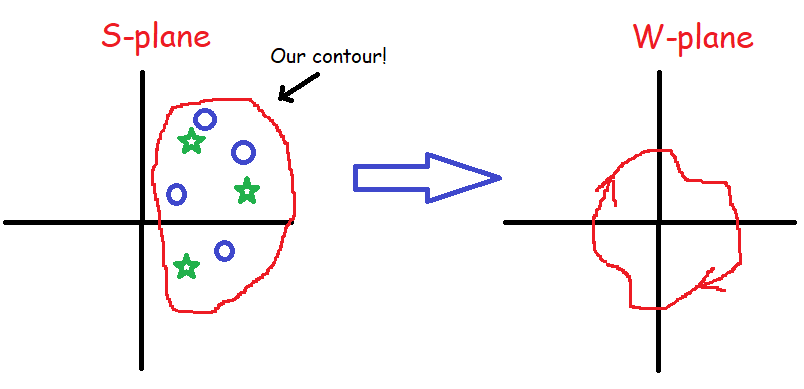
\includegraphics[scale= 0.4]{Images/sw.PNG}
    \caption{Mapping all of our values to create the plot}
    \label{Cauchy}
\end{figure}

Inside our contour we got four zeroes and tree poles. After we map all the values in the contour the plot in the w-plane is created. The plot surrounds the origin one time clockwise. This tells us that we got one more zero than pole inside our contour. If the plot was counterclockwise we would have had more poles than zeroes instead.

\subsection{Nyqvist theorem}
Nyqvist theorem will use this principle to find out if a system i stable or not. The Nyqvist theorem is graphical technique and will result in a Nyqvist plot. In the case of the a closed loop system the transfer function is defined as

\begin{equation*}
F(s) \ (1 + F(s)H(s))
\end{equation*}

That means if our denominator is equal to zero our system is unstable. That would be bad news!

To solve this we want to find out if we got any zeros in our right half plane. Therefore we surround our entire right half plane with a contour with infinite radius. We could map all these values to our denominator 
\begin{equation*}
1 + F(s)H(s)
\end{equation*}

but instead we are going to map our values to \begin{equation*}
F(s)H(s)
\end{equation*}

to make our lives easier. The will result of this will is the Nyqvist plot. Since we removed our +1 we a going to count the encirclements around -1 instead of the origin. In the picture you can take a look at this.


\begin{figure}[h!]
    \centering
    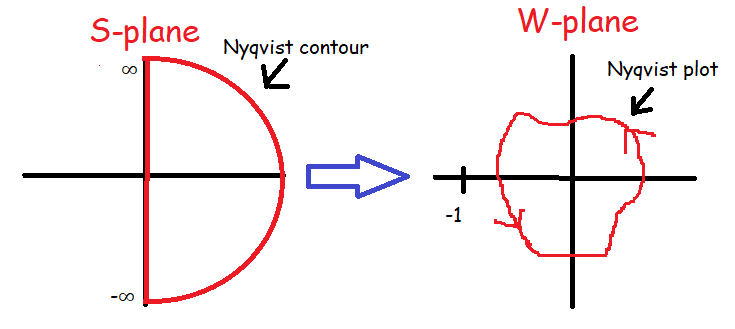
\includegraphics[scale= 0.4]{Images/nykv.PNG}
    \caption{Mapping all of our values from our Nyqvist contour to create the Nyqvist plot}
    \label{Nyqvist}
\end{figure}

Unfortunately this will only give us the difference between the number of zeroes and poles. To solve this will will utilise the equation $Z = N + P$. Where Z is the number of zeroes, N the number of clock wise encirclements and P is the number of poles in the open loop. In other words Nyqvist let us solve the closed-loop system with some help from the open-loop system.


This is how a Nyqvist plot is created and what i tell us about a transefer function. But since neither we or Haskell's map function can't compute with a infinite large input we have to find a way around this. We can instead focus on four important points and get a non-continuous plot. w=0, w=inf, w when we cross the real axis and w when we cross the imaginary axis. This will be enough for the most basic transfer functions you will see in the course.